\section{Annexes}
\subsection{Search tree}
In order to find the best possible move starting from a position, algorithms build search trees. 
Exemple with Tic-Tac-Toe : 
\begin{figure}[H]
	\centering
	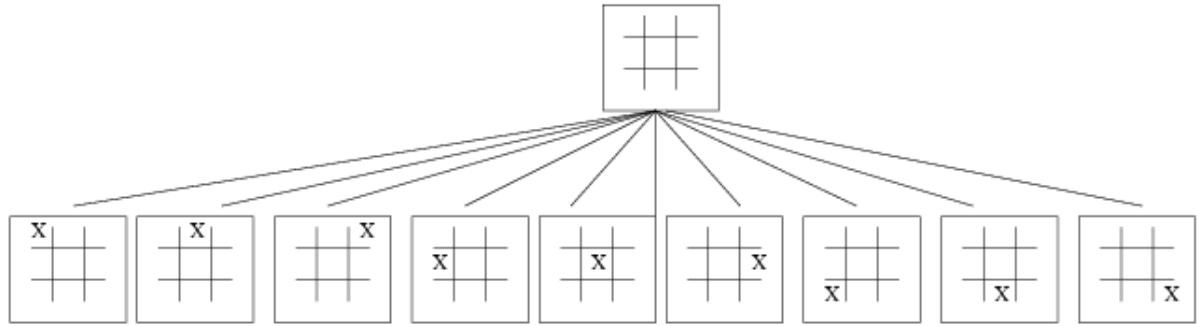
\includegraphics[height=1cm]{5_Annexes/img/Tree1.png}
	\caption{\label{fig:tree1}All possible moves starting from an empty board.}
\end{figure}
\noindent
For each positions, list all possible moves for the other player.

\begin{figure}[H]
	\centering
	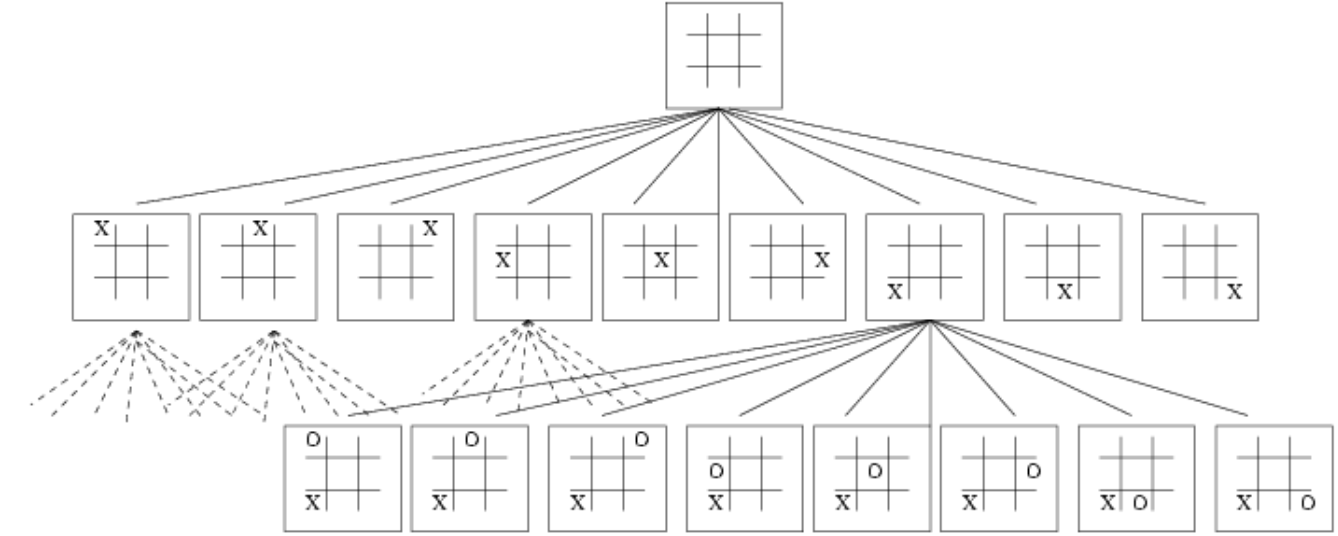
\includegraphics[height=1cm]{5_Annexes/img/Tree2.png}
	\caption{\label{fig:tree1}.}
\end{figure}
\noindent
\cite{images_annexes}
So far we've really seen no evaluation values. The way Minimax works is to go down a specified number of full moves (where one ``full move'' is actually a move by you and a move by your opponent), then calculate evaluation values for states at that depth. For this example, we're going to go down one full move, which is one more level. 
